\newpage
\section{Исходные данные}
\pagestyle{fancy}
\fancyhf{}
\rhead{Дипломная работа}
\lhead{Исходные данные}
\rfoot{\thepage}

\begin{longtable}[H]{|c|c|c|c|c|}
    \caption[Исходные данные]{Исходные данные} \label{tab:Исходные данные} \\
    \hline 
    №& Парамтр & Обозначение & Значение & Единица измерения\\ \hline
    \endfirsthead
    
    \multicolumn{5}{c}%
    {{ \tablename\ \thetable{}: Исходные данные}} \\
    \hline 
    №& Парамтр & Обозначение & Значение & Единица измерения\\ \hline
    \endhead
    \endfoot
    
    \hline \hline
    \endlastfoot
         \hline
        1 & Расчётная масса & $m$ & 180 & т\\ \hline
        2 & Масса пустова & $m_\text{пуст}$ & 80 & т\\
         & самолёта &  &  & \\ \hline
        3 & Масса топлива & $m_\text{т}$ & 90 & т\\ \hline
        4 & Масса комерческой & $m_\text{к}$ & 9 & т \\
         & нагрузки & & & \\ \hline
        5 & Площадь крыла & $S$ & 360 & м$^2$\\ \hline
        6 & Ширина хорды САХ & $b_a$& 14,5 & м\\ \hline
        7 & Размах крыла & $l$ & 25,6 & м\\ \hline
        8 & Стартовая тяга двигателя & $P_0$ & 180000 $\cdot 4$ & Н\\ \hline
        9 & Момент инерции самолёта& $J_z$ & 7,7 $\cdot 10^{6}$ & кг $\cdot$ м$^2$ \\ 
         & относительно оси OZ &  &  & \\ \hline
        10 & Эксплуатационная вертикальная & $n_y^\text{э}$ & 3,5 & -\\ 
         & перегрузка &  &  & \\ \hline
        11 & Максимальное значение & $q_{max}$ & $5 \cdot 10^5$ & Н/м$^2$\\ 
         & скоростного напора &  &  & \\ \hline
        12 & Предельное значение & $M_\text{пред}$ & 2,4 & -\\ 
         & числа Маха &  &  & \\ \hline
        13 & Относительное значение & $\bar{X}_{T}$ & 0,25& -\\ 
         & центровки самолёта &  &  & \\ \hline
        14 & Максимальный угол отклонения & $\delta_{\text{э}_{max}}$ & 25 &град \\ 
        & элевонов & & & \\ \hline
        15 & Нагрузка на крыло & $P_s$ & 4905 & ${\text{Н}}/{\text{м}^2}$ \\ \hline
        16 & Тяговооруженность & $\bar{P}_0$ & 0,408 & - \\ \hline

\end{longtable}

\begin{table}[H]
    \centering
    \caption{Коэффициенты, характеризующее продольное движение}
    \label{tab:Коэффициенты, характеризующее продольное движение}
    \begin{tabular}{|c||c|c|c|c|c|}
    \hline
        $M$ & $C_{y_0}^{\delta \text{э}}$ &$X_F$ & $X_{F_{\text{э}}}$ &$m_z^{\bar{\omega}_z}$ & $C_y^{\alpha}$ \\ \hline \hline
        0,03  & 0,8  & 0,285  & 0,6  & -3,25 & 2,3 \\ \hline
        0,25  & 0,8  & 0,285  & 0,6  & -3,25 &2,3 \\ \hline
        0,5  & 0,8  & 0,285  & 0,6  & -3,25 & 2,25\\ \hline
        0,75  & 0,8  & 0,288  & 0,6  & -3,36 & 2,26\\ \hline
        1  & 0,55  & 0,314  & 0,6  & -3,5 &2,28 \\ \hline
        1,25  & 0,45  & 0,39  & 0,76  & -3,3 &2,5 \\ \hline
        1,5  & 0,43  & 0,45  & 0,86  & -3,05 &2,97 \\ \hline
        1,75  & 0,43  & 0,45  & 0,86  & -2,9 & 3\\ \hline
        2  & 0,445  & 0,446  & 0,86  & -2,8 & 2,82\\ \hline
        2,25  & 0,44  & 0,44  & 0,86  & -2,75 & 2,75\\ \hline
        2,5  & 0,42  & 0,43  & 0,86  & -2,74 & 2,68\\ \hline
        2,75  & 0,38  & 0,43  & 0,86  & -2,74 & 2,61\\ \hline
        3  & 0,35  & 0,43  & 0,86  & -2,74 & 2,54\\ \hline
    \end{tabular}
\end{table}

\begin{table}[H]
    \centering
    \caption{Аэродинамичекские характеристики }
    \label{tab:Аэродинамичекские характеристики }
    \begin{tabular}{|c||c|c|c|c|}
    \hline
        $M$  & $A$  & $C_{x_{m}}$  & $C_y^{\text{доп}}$  & $C_y^{\alpha}$   \\ \hline \hline
        0,03  & 0,025  & 0,0175  & 0,85  & 2,3   \\ \hline
        0,25  & 0,025  & 0,0175  & 0,85  & 2,3  \\ \hline
        0,5  & 0,0247  & 0,01755  & 0,85  & 2,25  \\ \hline
        0,75  & 0,0242  & 0,0175655  & 0,84  & 2,26  \\ \hline
        1  & 0,0237  & 0,018  & 0,75  & 2,28  \\ \hline
        1,25  & 0,0256  & 0,0192  & 0,7  & 2,5   \\ \hline
        1,5  & 0,034  & 0,0223  & 0,65  & 2,97  \\ \hline
        1,75  & 0,038  & 0,022  & 0,63  & 3  \\ \hline
        2  & 0,042  & 0,02185  & 0,61  & 2,82   \\ \hline
        2,25  & 0,0445  & 0,0216  & 0,6  & 2,75   \\ \hline
        2,5  & 0,0475  & 0,0215  & 0,59  & 2,68  \\ \hline
        2,75  & 0,0498  & 0,02155  & 0,53  & 2,61   \\ \hline
        3 & 0,0498  & 0,0215  & 0,51  & 2,54   \\ \hline
    \end{tabular}
\end{table}

\begin{figure}[H]
    \center{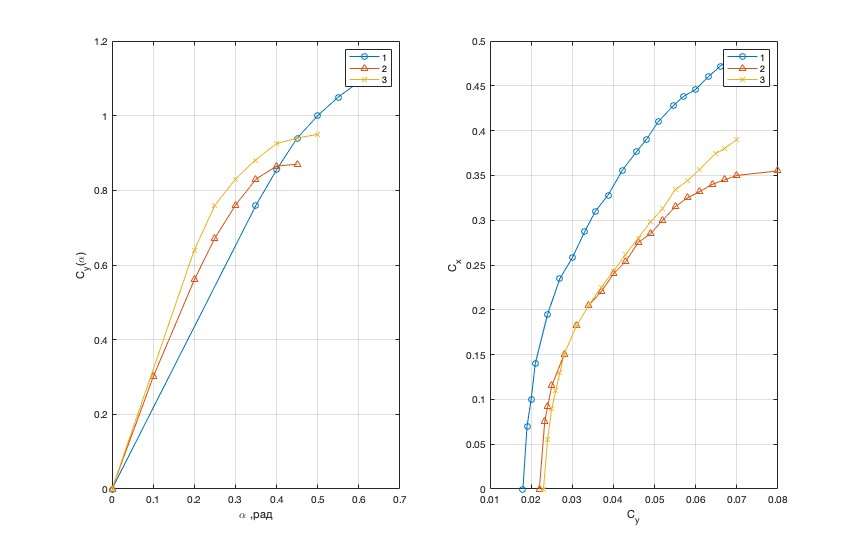
\includegraphics[width=\linewidth]{img/ПолярыДанные.jpg}}
    \caption{Аэродинамические характеристики на взлётно-посадочных
режимах;1-взлетный, 2-посадочный, 3-пробег с выпущенными
интерцепторами}
    \label{fig:ИД Взлёт посадка}
\end{figure}

\begin{center}
    Характеристики двигателя ДТРДФ:
\end{center}

\begin{longtable}[H]{|c|c|c|c|c|c|}
    \caption[Относительная тяга двигателя]{Относительная тяга двигателя, $\tilde{P}$} \label{tab:Относительная тяга двигателя} \\
    \hline 
    M/H, км& 0 & 3 & 6 & 9 &11 \\ \hline
    \endfirsthead
    
    \multicolumn{6}{c}%
    {{ \tablename\ \thetable{}: Относительная тяга двигателя, $\tilde{P}$}} \\
    \hline 
    M/H, км& 0 & 3 & 6 & 9 &11 \\ \hline
    \endhead
    \endfoot
    
    \hline \hline
    \endlastfoot
    \hline
        0,000  & 1,000 & 0,780 & 0,606 & 0,479 & 0,382  \\ \hline
        0,250  & 0,836 & 0,680 & 0,510 & 0,404 & 0,327  \\ \hline
        0,500  & 0,788 & 0,629 & 0,486 & 0,376 & 0,302  \\ \hline
        0,750  & 0,851 & 0,672 & 0,531 & 0,416 & 0,334  \\ \hline
        1,000  & 0,935 & 0,750 & 0,580 & 0,453 & 0,376  \\ \hline
        1,250  & 1,006 & 0,810 & 0,612 & 0,479 & 0,396  \\ \hline
        1,500  & 1,094 & 0,877 & 0,665 & 0,520 & 0,427  \\ \hline
        1,750  & 1,196 & 0,947 & 0,731 & 0,572 & 0,468  \\ \hline
        2,000  & 1,299 & 1,057 & 0,824 & 0,637 & 0,510  \\ \hline
        2,250  & 1,213 & 0,963 & 0,760 & 0,580 & 0,475  \\ \hline
        2,500  & 1,034 & 0,832 & 0,649 & 0,502 & 0,412  \\ \hline
        2,750  & 0,899 & 0,724 & 0,557 & 0,427 & 0,352  \\ \hline
        3,000  & 0,850 & 0,650 & 0,490 & 0,370 & 0,490  \\ \hline
\end{longtable}

\begin{longtable}[H]{|c|c|c|c|c|c|}
    \caption{Удельный расход топлива $C_{e}(M,H),\frac{\text{кг}}{\text{кгс} \cdot \text{час}}$} \label{tab:Удельный расход топлива} \\
    \hline 
    M/H, км& 0 & 3 & 6 & 9 &11 \\ \hline
    \endfirsthead
    
    \multicolumn{6}{c}%
    {{ \tablename\ \thetable{}: Удельный расход топлива $C_{e}(M,H),\frac{\text{кг}}{\text{кгс} \cdot \text{час}}$}} \\
    \hline 
    M/H, км& 0 & 3 & 6 & 9 &11 \\ \hline
    \endhead
    \endfoot
    
    \hline \hline
    \endlastfoot
    \hline
        0  & 0,88434 & 0,845814545 & 0,807289091 & 0,768763636 & 0,74308  \\ \hline
        0,25  & 0,9226 & 0,883673636 & 0,844747273 & 0,805820909 & 0,77987  \\ \hline
        0,5  & 0,9844 & 0,942263636 & 0,900127273 & 0,857990909 & 0,8299  \\ \hline
        0,75  & 1,07122 & 1,023866364 & 0,976512727 & 0,929159091 & 0,89759  \\ \hline
        1  & 1,16 & 1,12 & 1,068142727 & 1,014369091 & 0,97852  \\ \hline
        1,25  & 1,23161 & 1,184256364 & 1,136902727 & 1,089549091 & 1,05798  \\ \hline
        1,5  & 1,29341 & 1,24445 & 1,19549 & 1,14653 & 1,11389  \\ \hline
        1,75  & 1,33755 & 1,286585455 & 1,235620909 & 1,184656364 & 1,15068  \\ \hline
        2  & 1,38022 & 1,32805 & 1,27588 & 1,22371 & 1,18893  \\ \hline
        2,25  & 1,407 & 1,348786364 & 1,298222727 & 1,247659091 & 1,21395  \\ \hline
        2,5  & 1,42437 & 1,373402727 & 1,322435455 & 1,271468182 & 1,23749  \\ \hline
        2,75  & 1,43614 & 1,38718 & 1,33822 & 1,28926 & 1,25662  \\ \hline
        3 & 1,44 & 1,39 & 1,34 & 1,294 & 1,26 \\ \hline
\end{longtable}

\begin{figure}[H]
    \center{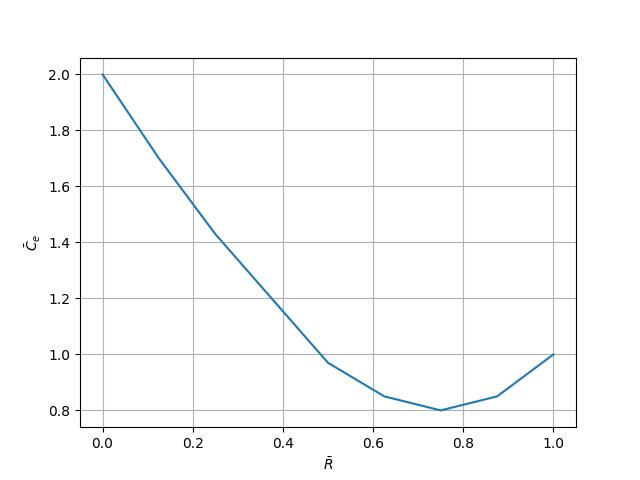
\includegraphics[width=\linewidth]{img/Дроссель.jpg}}
    \caption{Зависимость $\bar{C}_{e}(\bar{R})$}
    \label{fig:Ce}
\end{figure}

\begin{center}
    Выводы:
\end{center}

Все исходные данные, необходимые для расчетов, были взяты из
альбома исходных данных кафедры. Полученных данных достаточно для проведения всех необходимых расчетов. Корректировка и дополнение исходных данных не требуется.

